\section{Introduction}
\label{sec:introduction}

In Kathmandu Valley, the Bishnumati and Bagmati rivers carry the visible signature of rapid urbanization: floating plastics that threaten water sustainability where waste management cannot keep pace \cite{Pati2025}. The local scene scales globally, with on the order of a thousand rivers accounting for most riverine plastic emissions to the ocean \cite{Meijer2021}. Monitoring this flux is therefore a first-order environmental task, yet the dominant methods --- manual counting, net sampling, visual survey --- are slow, subjective, spatially sparse, and dangerous during the flood pulses that move the most litter \cite{Lieshout2020,Hurley2023}. Automated detectors already count substantially more items than human observers under identical conditions \cite{Lieshout2020}, which motivates a shift from episodic inspection to continuous observation (Fig.~\ref{fig:problem}).
% Problem diagram for the introduction (referenced as Fig.~\ref{fig:problem}).
\begin{figure}[!t]
\centering
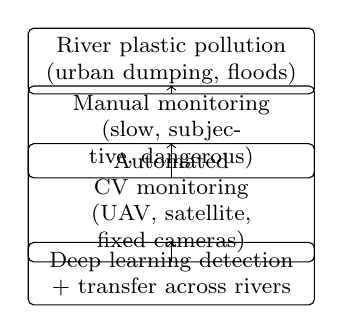
\begin{tikzpicture}[node distance=0.9cm, every node/.style={draw, rounded corners=2pt, text width=3.4cm, align=center, font=\footnotesize}]
\node (poll) {River plastic pollution\\(urban dumping, floods)};
\node (man) [below of=poll] {Manual monitoring\\(slow, subjective, dangerous)};
\node (auto) [below of=man] {Automated CV monitoring\\(UAV, satellite, fixed cameras)};
\node (dl) [below of=auto] {Deep learning detection\\+ transfer across rivers};
\draw[->] (poll) -- (man);
\draw[->] (man) -- (auto);
\draw[->] (auto) -- (dl);
\end{tikzpicture}
\caption{From river pollution evidence to automated monitoring: manual limits motivate continuous computer-vision observation, and deep learning must transfer across rivers to be useful.}
\label{fig:problem}
\end{figure}


Computer vision reframes rivers as scannable surfaces. Unmanned aerial vehicles deliver centimetre detail over reaches \cite{Maharjan2022,Jakovljevic2020}; satellites revisit whole basins at coarser grains \cite{SoleGomez2022,Mohsen2023}; bridge and bank cameras watch fixed cross-sections around the clock \cite{Lieshout2020,Reinhardt2024}; phones and citizen observers extend coverage where infrastructure is absent \cite{JiaFrontiers2023,Tharani2021}. Deep learning converts these pixels into detections, masks, and counts with rapidly maturing accuracy \cite{Jia2023}. The base study for this review exemplifies the state of the art: a controlled comparison of detection and segmentation under three training strategies with cross-river transfer tests on novel Nepali datasets \cite{Pati2025}.

What remains unanswered is generalization. Prior syntheses catalogue platforms \cite{Marye2025} and architectures \cite{Jia2023} but do not systematically ask whether a model trained on one river, sensor, or season works on another. This review fills that gap as the first generalization-centered synthesis of deep-learning waste detection across riverine environments. It contributes: (i) an evidence-graded corpus of 50 studies spanning UAV, satellite, fixed, handheld, surface-vehicle, and (by documented absence) underwater sensing; (ii) a four-level generalization grading applied uniformly, separating demonstrated transfer from claimed robustness; (iii) a replication record for the base study's findings across independent rivers and continents; and (iv) a gap inventory oriented to Nepal-like, resource-constrained settings where transfer learning matters most.
